\begin{flushright} {\tiny {\color{gray} \tt benchmark\_hollowsphereintpress.tex}} \end{flushright}
%~~~~~~~~~~~~~~~~~~~~~~~~~~~~~~~~~~~~~~~~~~~~~~~~~~~~~~~~~~~~~~~~~~~~~~~~~~~~~~~~~~~~~~~~~~~~~~~~~~

This benchmark was inspired by the one at \url{XXX}. 
A homogenous hollow sphere (internal radius $a$, external radius $b$) is made of an elastic 
perfectly plastic material (characterised by the Young's modulus $E$ and the Poisson ratio $\nu$, 
yield stress $\sigma_y$). The yield criterion in von Mises. 
Starting from an initial stress-free state the internal pressure rises from $0$ to $p$.

\begin{center}
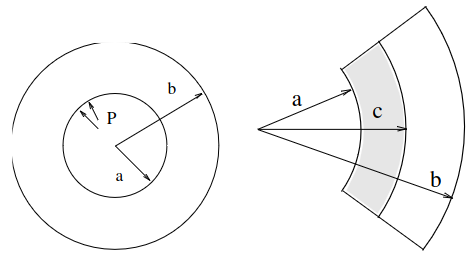
\includegraphics[width=7cm]{images/benchmark_hollowsphereintpress/sphere}\\
{\captionfont Left: geometry and applied load. Right: illustration of the plastic zone
growing from the internal surface.}
\end{center}

Since the body's geometry and the loading present a spherical symmetry, and since the material
behaviour is isotropic the solution is built in spherical coordinates $(r,\theta,\phi)$.
The displacement field is then given by
\begin{eqnarray}
u_r &=& h(r) \nn\\
u_\theta &=& 0 \nn\\
u_\phi &=& 0  \nn
\end{eqnarray}
The strain tensor in spherical coordinates is given by

\begin{eqnarray}
\varepsilon_{rr} 
&=& \frac{\partial u_r}{\partial r} \nonumber\\
\varepsilon_{\theta\theta} 
&=& \frac{u_r}{r} + \frac{1}{r} \frac{\partial u_\theta}{\partial \theta}  \nonumber\\
\varepsilon_{\phi\phi} 
&=& \frac{1}{r \sin\theta} \frac{\partial u_\phi}{\partial \phi} +
\frac{u_r}{r} +\frac{u_\theta \cot \theta}{r} \nonumber\\
\varepsilon_{\theta r} = \varepsilon_{r\theta}   
&=& \frac{1}{2} \left( r \frac{\partial}{\partial r} (\frac{u_\theta}{r} ) 
+\frac{1}{r} \frac{\partial u_r}{\partial \theta} \right) \nonumber\\
\varepsilon_{\phi r} = \varepsilon_{r\phi}      
&=&  \frac{1}{2} \left(  \frac{1}{r \sin\theta} \frac{\partial u_r}{\partial \phi} 
+ r \frac{\partial }{\partial r} (\frac{u_\phi}{r}) \right)  \nonumber\\
\varepsilon_{\phi \theta} = \varepsilon_{\theta\phi} 
&=& \frac{1}{2} \left( \frac{\sin \theta}{r} \frac{\partial }{\partial \theta} (\frac{u_\phi}{\sin\theta}) + \frac{1}{r \sin\theta} \frac{\partial u_\theta}{\partial \phi}    \right) \nonumber
\end{eqnarray}
which leads to:
\begin{eqnarray}
\varepsilon_{rr}  &=& \frac{\partial u_r}{\partial r} =f_2(r) \nonumber\\
\varepsilon_{\theta\theta} &=& \frac{u_r}{r} =g_2(r)  \nonumber\\
\varepsilon_{\phi\phi} &=& \frac{u_r}{r} =g_2(r)  \nonumber\\
\varepsilon_{\theta r} = \varepsilon_{r\theta}   
&=& 0 \nn\\ 
\varepsilon_{\phi r} = \varepsilon_{r\phi}      
&=& 0 \nn\\ 
\varepsilon_{\phi \theta} = \varepsilon_{\theta\phi} &=& 0 \nn
\end{eqnarray}
because we also have $\partial_\theta \rightarrow 0$ and $\partial_\phi \rightarrow 0$,
Then
\[
\vec{\nabla}\cdot\vec{u} = \frac{\partial u_r}{\partial r} + 2 \frac{u_r}{r}
\]


Finally the stress tensor is given by 
\[
{\bm \sigma}=\lambda (\vec{\nabla}\cdot\vec{u}) {\bm 1} +2\mu {\bm \varepsilon}(\vec{u}) 
\]

\begin{eqnarray}
\sigma_{rr} &=&   \lambda \left(  \frac{\partial u_r}{\partial r} + 2 \frac{u_r}{r} \right)
+ 2 \mu \frac{\partial u_r}{\partial r} =f_1(r) \nn\\
\sigma_{\theta\theta} &=& \lambda \left(  \frac{\partial u_r}{\partial r} + 2 \frac{u_r}{r} \right)
+ 2 \mu \frac{u_r}{r} =g_1(r)\nn\\
\sigma_{\phi\phi} &=&  \lambda \left(  \frac{\partial u_r}{\partial r} + 2 \frac{u_r}{r} \right)
+ 2 \mu \frac{u_r}{r} =g_1(r)\nn\\
\sigma_{r\theta} &=& 2\mu \varepsilon_{r\theta} = 0 \nn\\ 
\sigma_{r\phi} &=& 2\mu\varepsilon_{r\phi} = 0 \nn\\ 
\sigma_{\theta\phi} &=& 2\mu  \varepsilon_{\theta\phi} = 0 \nn\\ 
\end{eqnarray}

The strong form of the PDE that governs force balance in a medium is given by
\[
\vec\nabla \cdot {\bm \sigma} + \vec{f} = \vec{0}
\]
In this case $\vec{f}=\vec{0}$.
The divergence of the stress tensor in spherical coordinates is given 
by\footnote{\url{https://en.wikipedia.org/wiki/Linear_elasticity}}:
\begin{eqnarray}
\frac{\partial \sigma_{rr}}{\partial r} + \frac{1}{r} \frac{\partial \sigma_{r\theta}}{\partial \theta}
+\frac{1}{r \sin \theta} \frac{\partial \sigma_{r\phi}}{\partial \phi}
+\frac{1}{r} (2\sigma_{rr} -\sigma_{\theta\theta} -\sigma_{\phi\phi} 
+ \sigma_{r\theta} \cot \theta) &=& 0 
\\
\frac{\partial \sigma_{r\theta}}{\partial r}+
\frac{1}{r}\frac{\partial \sigma_{\theta\theta}}{\partial \theta}+
\frac{1}{r \sin \theta} \frac{\partial \sigma_{\theta\phi}}{\partial \phi}
+\frac{1}{r} \left(
(\sigma_{\theta\theta}-\sigma_{\phi\phi})\cot \theta + 3 \sigma_{r\theta} 
\right)&=& 0 
\\
\frac{\partial \sigma_{r\phi}}{\partial r}+
\frac{1}{r}\frac{\partial \sigma_{\theta\phi}}{\partial \theta}+
\frac{1}{r \sin \theta} \frac{\partial \sigma_{\phi\phi}}{\partial \phi}
+\frac{1}{r} \left(
2\sigma_{\theta\phi} \cot\theta + 3 \sigma_{r\phi}
\right)&=& 0 
\end{eqnarray}
Again, using $\partial_\theta \rightarrow 0$ and $\partial_\phi \rightarrow 0$
and remembering that $\sigma_{\theta\theta}=\sigma_{\phi\phi}$
we find that the lhs of the second and third lines are identically zero,
and the first line becomes simply
\[
\frac{\partial \sigma_{rr}}{\partial r} + 
\frac{1}{r} (2\sigma_{rr} -\sigma_{\theta\theta} -\sigma_{\phi\phi} ) = 0 
\]

---- I need to reconcile above with below --- July 23rd, 2024

The equilibrium, the static and kinematic boundary conditions can be expressed as:


\begin{eqnarray}
\frac{d\sigma_{rr}}{dr} + \frac{2}{r}(\sigma_{rr}-\sigma_{\theta\theta})&=&0 \\
\sigma_{rr}(r=a) &=& -p\\
\sigma_{rr}(r=b) &=& 0 \\
\varepsilon_{rr} &=& \frac{du_r}{dr} \\
\varepsilon_{\theta\theta} &=& \frac{u_r}{r} 
\end{eqnarray}
The elastic constitutive equations also write\footnote{\url{
https://en.wikipedia.org/wiki/Linear_elasticity}}:
\[
\varepsilon_{ij} 
= \frac{1}{2\mu} \sigma_{ij}  - \frac{\nu}{E} \delta_{ij} \sigma_{kk}
= \frac{1}{E} \left[ (1+\nu)\sigma_{ij} -\nu\delta_{ij}\sigma_{kk}  \right]
\]
We have
\[
\sigma_{kk} 
= \sigma_{rr} + \sigma_{\theta\theta} + \sigma_{\phi\phi}  
= \sigma_{rr} + 2\sigma_{\theta\theta} 
\]
so that explicitely 
\begin{eqnarray}
E \varepsilon_{rr} &=&    (1+\nu)\sigma_{rr} -\nu ( \sigma_{rr} + 2\sigma_{\theta\theta}    )\nn \\
E \varepsilon_{\theta\theta} &=&    (1+\nu)\sigma_{\theta\theta} -\nu( \sigma_{rr} + 2\sigma_{\theta\theta}) \nn\\
E \varepsilon_{\phi\phi} &=&   (1+\nu)\sigma_{\phi\phi} -\nu( \sigma_{rr} + 2\sigma_{\theta\theta}    ) \nn
\end{eqnarray}
or (removing the useless third line),
\begin{eqnarray}
E \varepsilon_{rr} &=& (\sigma_{rr}-2 \nu \sigma_{\theta\theta}) \nn\\
E \varepsilon_{\theta\theta} &=& \sigma_{\theta\theta} (1-\nu) - \nu \sigma_{rr}
\end{eqnarray}
After replacing strain by its expression as a function of displacement, 
it comes (using $\lambda = E \nu /(1-2\nu)/(1+\nu) )$:
\begin{eqnarray}
\sigma_{rr} &=& \frac{\lambda}{\nu}
\left((1-\nu)\frac{du_r}{dr} + 2\nu \frac{u_r}{r}\right) \nn\\
\sigma_{\theta\theta} &=& \frac{\lambda}{\nu}
\left(\nu \frac{du_r}{dt} + \frac{u_r}{r}\right)
\end{eqnarray}
These two equations can be introduced in the equilibrium equation, leading to :
\[
\frac{d^2 u_r}{dr^2} + \frac{2}{r} \frac{du_r}{dr} -\frac{2}{r^2}u_r = 0
\]
The solution of this equation is :
\[
u_r(r) = C_1 r + \frac{C_2}{r^2}
\]
By replacing $u_r$ in the preceding expressions, it comes:
\begin{eqnarray}
\sigma_{rr} &=& \frac{\lambda}{\nu}
\left((1+\nu)C_1 - 2(1-2\nu)\frac{C_2}{r^3}\right) \nn\\
\sigma_{\theta\theta} &=& \frac{\lambda}{\nu}
\left((1+\nu)C_1 + (1-2\nu)\frac{C_2}{r^3}\right) 
\end{eqnarray}
The integration constants $C_1$ and $C_2$ can be determined from the boundary conditions:
\begin{eqnarray}
\sigma_{rr}(r=b)=0 &\Rightarrow& 
C_2=\frac{1+\nu}{2(1-2\nu)}b^3 C_1 \\
\sigma_{rr}(r=a)=-p &\Rightarrow& 
C_1=\frac{1-2\nu}{E}\frac{a^3}{b^3-a^3}p
\end{eqnarray}
so that in the end:
\begin{eqnarray}
\sigma_{rr} &=& -\frac{a^3}{b^3-a^3} \left( \frac{b^3}{r^3}-1 \right) p \nn\\
\sigma_{\theta\theta}=\sigma_{\phi\phi} &=& \frac{a^3}{b^3-a^3} \left( \frac{b^3}{2r^3}+1 \right) p \nn\\
u_r &=& \frac{a^3}{b^3-a^3}
\left( (1-2\nu)r+(1+\nu)\frac{b^3}{2r^2}  \right)\frac{p}{E}
\end{eqnarray}

Both criteria are insensitive to hydrostatic pressure. They resulting value is 
then not affected if a
spherical tensor is added. In the present case, if the 
diagonal $\sigma_{rr},\sigma_{\theta\theta},\sigma_{\phi\phi})$ is subtracted from the actual
tensor the new tensor is simply uniaxial, the only non zero component 
being $\sigma_{rr}-\sigma_{\theta\theta}$ , which is then
the value of both von Mises and Tresca criteria. Using the solution 
of the preceding question, this value
can be evaluated in the elastic regime, as :
\[
\sigma_{\theta\theta} - \sigma_{rr} = \frac32 \frac{a^3}{b^3-a^3} \frac{b^3}{r^3} p
\]
The plastic yield is reached when $(\sigma_{\theta\theta} - \sigma_{rr})$, 
increasing function of $p$, is equal to $\sigma_y$ , the yield limit
in onedimensional tension. The initial plastic zone is then located in $r=a$, 
and the value of the pressure $Pe$ is :
\[
P_e = \frac23 \left( 1 - \frac{a^3}{b^3} \right)\sigma_y
\]

Let us recall Eq.~\eqref{eq:I2s123}:
\[ 
{\III}_2({\bm \tau}) = \frac{1}{6}\left[(\sigma_{1}-\sigma_{2})^2 + (\sigma_{2}-\sigma_{3})^2 
+ (\sigma_{1}-\sigma_{3})^2 \right] 
\]
then we have
\[ 
{\III}_2({\bm \tau}) 
= \frac{1}{6}\left[(\sigma_{rr}-\sigma_{\theta\theta})^2 
+ (\sigma_{\theta\theta}-\sigma_{\phi\phi})^2 
+ (\sigma_{rr}-\sigma_{\phi\phi})^2 \right] 
=
\frac{1}{6}\left[(\sigma_{rr}-\sigma_{\theta\theta})^2 
+ (\sigma_{rr}-\sigma_{\theta\theta})^2 \right] 
=\frac13 (\sigma_{rr}-\sigma_{\theta\theta})^2 
\]
or, 
\[
\sqrt{{\III}_2({\bm \tau}) } = \frac{1}{\sqrt{3}} |\sigma_{rr}-\sigma_{\theta\theta}|
\]
and the von Mises criterion writes (see Eq.~\eqref{vmcrit}):
\[
\sqrt{3} \sqrt{{\III}_2({\bm \tau}) } - \sigma_y = 0
\]
or,
\[
|\sigma_{rr}-\sigma_{\theta\theta}|
- \sigma_y = 0
\]
Let us compute the lhs:

\begin{eqnarray}
\sigma_{rr}-\sigma_{\theta\theta}
&=& 
-\frac{a^3}{b^3-a^3} \left( \frac{b^3}{r^3}-1 \right) p 
-\frac{a^3}{b^3-a^3} \left( \frac{b^3}{2r^3}+1 \right) p \nn\\
&=& 
-\frac{a^3}{b^3-a^3}\frac32 \frac{b^3}{r^3}  p 
\end{eqnarray}
Since $b>a$ and $p>0$ then 
\[
| \sigma_{rr}-\sigma_{\theta\theta} |=
\frac{a^3}{b^3-a^3}\frac32 \frac{b^3}{r^3}  p 
\]

The plastic yield is reached when $(\sigma_{\theta\theta} - \sigma_{rr})$, 
increasing function of $p$, is equal to $\sigma_y$ , the yield limit
in onedimensional tension. The initial plastic zone is then located in $r=a$, 
and the value of the pressure $Pe$ is :
\[
P_e = \frac23 \left( 1 - \frac{a^3}{b^3} \right)\sigma_y
\]










